\documentclass[sim-use, blue_items]{checklist}
\usepackage{gensymb}
\usepackage{textcomp}

\logo{logo_white/boeing.png}
\title{Normal Procedures}
\subtitle{Boeing \\ 747-200}
\version{Version: 1.0 \\ \today}

\begin{document}

\begin{checklist}{Cockpit Safety Inspection - F/E}
	\note{Perform on originating trip or crew change\\when electrical and pneumatic power isn't applied to the aircraft.}
	\specialitem{Windshield Wiper Switches}{Off}
	\specialitem{Alternate Flap Switches}{Off}
	\specialitem{Landing Gear Lever}{Down \& In}
	\specialitem{Radar}{Off}
	\specialitem{Transponder Mode Switches}{STBY}
	\specialitem{Galley Power Bus Switches}{Off}
	\specialitem{Electric \& Air Driven Hydraulic Pump Switches}{Off}
	\specialitem{Fuel Jettison Panel Cover}{Closed}
\end{checklist}

\begin{checklist}{Preliminary Cockpit Preparation - F/E}
	\note{F/E'S STATION}
	\item{Circuit Breakers}{Check}
	\specialitem{Standby Power Switch}{Off}
	\item{Battery Switch}{On}
	\specialitem{DC Meters Selector}{APU Batt}
	\specialitem{APU Master Switch}{On}
	\specialcondition{APU Fire Warning and Squib Checks}{
		\item{APU Fire Switch}{in, discharge light extinguished}
		\item{APU Squib Test}{Perform, Check Light}
		\item{APU Fire Test A \& B}{Perform, Check Fire Warning Lights \& Bell}
		\item{APU Fault Test A \& B}{Perform, Check Fault Lights}
	}
	\specialitem{APU}{Start}
	\specialitem{APU or External Electrical Power}{Establish}
	\specialcondition{Standby and Essential Power Checks}{
		\item{Warning Flags on N1 and EGT}{Check Displayed}
		\item{Standby Power Switch}{Manual On}
		\item{Standby Power On Light}{Check Illuminated}
		\item{Warning Flags on N1 and EGT}{Check Out Of View}
		\item{Standby Power Switch}{Normal}
		\item{Standby Power On Light}{Check Extinguished}
		\item{Essential Power Switch}{Check Normal, Ess bus off lights extinguished}
	}
\end{checklist}

\begin{continuedchecklist}
	\specialcondition{DC Power Checks}{
		\item{APU Battery}{Check 25V - 36V}
		\item{Battery and TRs}{Check 25V - 32V}
		\item{TRs}{Check Positive DC AMP}
	}
	\specialitem{DC Bus Isolation Switches}{Close, Check Open Lights Extinguished}
	\specialcondition{Air Conditioning and Pneumatic Systems Checks} {
		\item{APU Bleed}{Open}
		\item{Duct Isolation Switches}{Check Open}
		\item{Duct Pressure L \& R}{Check Normal}
		\item{Gasper Fan}{As Desired}
		\item{Suppl Vent Fans}{Off}
		\item{Recirc Fans}{1 Off, 2,3,4 On}
		\item{All PACK Control Switches}{Check Auto}
		\item{Zone Temp Switches}{Check Auto, Overheat Lights Extinguished}
		\item{Trim Air Switch}{Open}
		\item{No. 1 PACK Selector}{Press, check Bypass more than 0.25 over full COOL,\\inlet \& exit doors in full COOL position}
		\item{No. 1 PACK Valve Switch}{Place Open, Check Pack trip Light Exting.}
		\item{No. 2 \& 3 PACKs}{Repeat Steps}
		\item{All PACKs}{Check ACM Outlet \& Compressor Discharge Temperatures Normal}
	}
	\note{PILOTS' STATION}
	\specialitem{Forward and Overhead Panel Indicator Lights}{Test}
	\specialitem{Radio Master Bus Switches}{On}
	\specialitem{INS Systems}{Select STBY, Perform Tests, Load Position,\\Select Align, Check Performance}
	\specialitem{Wheel Well Fire Detector}{Test, Check Fire Warning Lights}
	\specialitem{Cockpit Voice Recorder}{Test, Check Double Bounce}
	\specialitem{Emergency Lights}{Off, Check Unarmed Light Illuminated}
	\item{No Smoking (and Fasten Seatbelts) Signs}{On}
	\specialitem{Stall Warning Test}{Perform, Check PWR Off light Extinguished,\\disc rotates and Stick Shaker Vibrates,\\Check Light Illuminated once Switch is released}
	\item{Mach/Airspeed Warning Test}{Perform, Check Clacker Sound}
	\condition{Once INS No. 1 Alignment Status $\le$ 8} {
		\item{Over Rotation Warning}{Test, Check Disc Rotates and Stick Shaker Vibrates}
	}
	\specialitem{Wing Anti-Ice}{Off}
\end{continuedchecklist}

\begin{continuedchecklist}
	\specialcondition{Probe Heat Checks} {
		\item{Probe Heat Switches}{Check Off, check warning lights illuminated}
		\item{Probe Heat Switches}{TAT Test, check TAT Probe Lights extinguish}
		\item{Probe Heat Switches}{On, check warning lights extinguish}
		\item{Probe Heat Switches}{Off}
	}
	\specialcondition{Window Heat Checks} {
		\item{Window Heat Switches}{On}
		\item{Power Lights}{On, check L1 \& R1 illuminate}
		\item{If L1 \& R1 don't illuminate}{Press Power Test, Check Illumination again}
		\item{Window Heat Switches}{Off}
	}
	\specialitem{Navigation Light Switch}{On}
	\item{Annunciator Lights}{Check} % Check!
	\item{Engine Instruments}{Normal, Check Power Failure Flags hidden,\\maximum indication pointers at correct setting}
	\specialitem{Total and Static Air Temperatures}{Check Failure Flags hidden,\\temperatures comparable}
	\specialitem{Takeoff Warning Horn}{Check}
	\specialitem{EPRL System}{Check warning flags out of view}
	\specialitem{EPRL System Test}{Perform in all Modes, check Response on Centre Panel}
	\specialitem{Oxygen Emergency Levers}{Check Off at all Stations} %Really?
	\specialitem{Crew Oxygen Control Valve}{Check Open, Pressure in Green Band}
	\note{F/E'S STATION}
	\item{F/E Panel Indicator Lights}{Test}
	\specialitem{Galley/Lavatory Exhaust Fan}{Set Auto}
	\item{Galley Power Bus Switches}{On, Check Trip Off Lights Exting. \& Load Limits not exceeded}
	\item{Crew and Passenger Oxygen}{Check Pressure Adequate} %Crew??
	\item{Passenger Oxygen Switch}{Check Norm \& guarded, on Light extinguished}
	\condition{AC Electrical System Checks} {
		\item{GEN OPEN \& CSD OIL Lights}{Check Illuminated} %CSD Oil Press?
		\item{KW Load Meters}{Check Indicating Zero}
		\item{FIELD OFF \& GEN BRG FAILURE Lights}{Check Extinguished}
		\item{CSD Disconnect Switches}{Check Guards Down}
		\item{CSD Oil Temperature}{Check Indications Normal}
	}
	\item{Oil System}{Check Quantities adequate, Temperatures normal, Pressures Zero\\and FILTER BY PASS Lights extinguished}
\end{continuedchecklist}

\begin{continuedchecklist}
	\specialcondition{Fuel System Checks} {
		\item{Fuel Quantity Test}{Hold Switch, Wait until ERR 0 is displayed}
		\item{Fuel Indications}{Check ERR 4 and All Segments, then total fuel capacity is displayed}
		\item{Fuel Indications}{Check Return to original values after test is finished}
		\item{Fuel Quantity}{Check Correct Amount on Board}
		\item{Fuel Boost \& Override Pumps}{Turn only fwd, then only aft on, check Lights}
		\item{Fuel Crossfeed Valves}{Toggle, Check transit lights illuminate and extinguish}
		\item{Reserve Valves}{Open \& Close, check lights illuminate and extinguish}
		\item{ENG VALVE Lights}{Check illuminated dim}
		\item{Fuel Heat Switches}{Check in CLOSED/OFF, Check ICING \& Heater Lights extinguished}
		\item{Scavenge Pump Switch}{On if Fuel in centre tank,\\Check LOW Pressure Lights extinguish, Off}
		\item{Fuel Pressure Indicators}{Check Zero}
		\item{ENG Fuel Temperature Indicators}{Press for each Engine, check On Light \& Temperature} %Reset Fuel Used?
	}
	\condition{Cabin Altitude Control Module Checks} {
		\item{Pressurization Rate Selector}{Set to Index}
		\item{Flight/Cabin Altitude Selector}{Set to 1000ft above cruise altitude on FLT scale}
		\specialitem{Altimeter}{Set, Check correct altitude indication}
		\item{BARO SET indicator \& Altimeter}{Set to standard Pressure}
		\specialitem{Pressurization Mode Switch}{Check AUTO}
		\specialitem{Rate Limit Test Switch}{hold, check Outflow valves close and rate limit light}
		\specialitem{Rate Limit Test Switch}{release, check Outflow valves open}
		\specialitem{Pressurization Mode Switch}{Set MAN, Check Valves Stop}
		\specialitem{Pressurization Mode Switch}{Set AUTO, Check Valves Open}
	}
	\item{Engine Bleed Switches}{Open, check valve closed lights illuminated,\\high stage \& Overheat Light extinguished}
	\specialitem{PACK ACM \& Compressor Discharge Temperatures}{Check Comparable \& Normal}
	\specialcondition{Equipment Cooling System Checks} {
		\item{Blower Switch}{Check Norm}
		\item{NO AIR FLOW Light}{Check Extinguished}
		\item{Equipment Cooling Valve Switch}{Check Norm \& Guarded}
		\item{Smoke Detector Test}{Perform, check light illuminates}
	}
	\specialitem{Squib Circuits}{Test Left \& Right Bottle, Check Squib OK Lights, then Off}
	\specialitem{Aft Cargo Heat System}{Test, Check On Light Illum., overheat light Exting., then Off}
\end{continuedchecklist}

\begin{continuedchecklist}
	\specialcondition{Lower Cargo Fire Protection Checks} {
		\item{Fire Detector Switches}{Check BOTH}
		\item{Compartment Select Switch, Discharge Switch \& Discharge Lights}{Check Off \& Guarded}
		\item{Detector Test Switch "A"}{Hold, check 3 Detector A Lights illuminate}	
		\item{Detector Test Switch "B"}{Hold, check 3 Detector B Lights illuminate}	
		\item{Both Detector Test Switches}{Hold, check Fire Warning Lights illuminate}
		\item{Fire Warning Lights}{Check Extinguish after Release}
		\item{Squib Test Switches 1 \& 2}{Press, Check Lights}
	}
	\specialcondition{Engine Fire Detection and Nacelle Temperature Indication Checks} {
		\item{All Engine Fire Switches}{Check In, discharge Lights extinguished}
		\item{All Nacelle Fire Detector Switches}{Check Both}
		\item{Test Switches Dual}{Place in Fire \& Fault, Check Fire Warning Lights and Bell,\\Nacelle Temperature Indications over 8}
		\item{Test Switches A \& B}{Place in Fire \& Fault, Check Fault Warning Lights,\\Nacelle Temperature Indications over 8}
	}
	\condition{Hydraulic System Checks} {
		\item{Normal Brake Source Switch}{Check in Prim Sys 4 and guarded}
		\item{SEC SYS 1 light}{Check Extinguished}
		\item{Brake \& Brake Source LOW PRESS Lights}{Check Illuminated}
		\item{Hydraulic Quantity Test Switch}{Press, Check Needles Drive toward zero \& return}
		\item{HYD QTY indicators}{Check in green Band}
		\item{Hydraulic LOW QTY, OVERHEAT Lights}{Check Extinguished}
		\item{System Temperatures}{Check All Roughly the Same}
		\item{Engine Driven Pump Switches}{Check Normal, Hydraulic LOW PRESS Light illum.}
	}
	\specialitem{Engine Vibration Indicators}{Check Zero}
	\specialitem{Total Air Temperature Indicator}{Check Off Flag hidden, comparable to Pilots' indicator}
	\specialitem{F/E Clock}{Set}
	\specialitem{Body Gear Steering Light}{Check Press, Body unlocked Lights Exting.}
	\specialitem{Leading Edge Flap Indicator Module}{Check Lights agree with LE Flap Position}
	\specialcondition{Landing Gear Annunciator Module Checks} {
		\item{Gear and Tilt PRIM \& ALT Switches}{Press, Check lights Turn Illum.}
		\item{Door PRIM \& ALT Switches}{Press, Check lights Agree with Door Positions}
	}
	\specialitem{Brake Temperature Monitor Test}{Press, Check All Indicators Full \&\\Overheat Warning Lights Illum.}
	\specialitem{Brake Temperature Monitor Test}{Release, Check All Indicators Normal \&\\Overheat Warning Lights Exting.}
	\specialitem{Wing Leading Edge Overheat System Test 1 \& 2}{Perform, check Overheat Lights}
	\specialitem{Generator Annunciator Module}{Press READ Switch, check lights stay extinguished}
	\specialitem{Door Annunciator Module}{Check Lights correspond to system Status}
\end{continuedchecklist}

\begin{continuedchecklist}
	\specialcondition{Flight Recorder Setup}{
		\item{Trip Number}{Set}
		\item{Flight Recorder Switch}{Hold Test, check Lights}
	}
	\specialitem{Anti-Skid Ground Mode PRIM \& ALT TEST}{Perform, check Light}
	\item{Potable Water}{Check desired Quantity}	
	\specialitem{F/E Life Vest \& Smoke Goggles}{Check Stowed}
	\item{Oxygen Mask, Hose and Regulator}{Checked, On, 100\%}
	\item{Crew Emergency Hatch}{Check Closed \& Locked, Escape Devices Stowed}
	\specialitem{Cockpit Emergency Equipment \& Upper Deck Door Slide}{Check}
\end{continuedchecklist}

\begin{checklist}{Cockpit Preparation - C \& F/O}
	\specialitem{Life Vest \& Smoke Googles}{Stowed}
	\item{Oxygen}{Checked, On, 100\%}
	\specialitem{Static Source Selectors}{Normal} %Where?
	\specialitem{Flight Control Power Switches}{On, Valve Closed lights extinguished}
	\item{Auto Brake Arm Switch}{Off}
	\specialitem{Yaw Damper Switches}{Engaged}
	\specialitem{Anti-Skid Switch}{On \& Guarded, check ANTI-SKID annunciator extinguished}
	\item{Body Gear Steering Switch}{Arm}
	\item{Ignition Switches}{Off, check Valve open lights extinguished}
	\specialitem{INS Mode Switches}{Align}
	\item{Compasses}{Slaved}
	\condition{If Synchronization indicator not aligned}{
		\item{DG/SLAVED Switch}{DG Momentarily}
		\item{DG/SLAVED Switch}{Return to Slaved}
	}
	\condition{If Synchronization indicator still not aligned}{
		\item{SET HDG Switch}{Use to align indicator}
	}
	\specialitem{Alternate Gear Extension Switches}{Off}
	\specialitem{HF Radios}{Set as Required (USB), not within 50ft of refueling}
	\specialitem{Standby Ignition Switch}{Norm}
	\specialitem{Emergency Lights}{Armed, check unarmed light extinguished}
	\item{Cabin Signs}{Check no smoking,\\fasten seatbelts and flt dk door rel lights illuminated}
	\item{Alternate Flap Switches}{Off}
	\specialitem{Nacelle Anti-Ice Switches}{Off}
	\item{Probe Heat Switches}{On}
	\item{Window Heat Switches}{On}
\end{checklist}

\begin{continuedchecklist}
	\item{Cockpit Lights}{Set as Desired}
	\item{Radio/INS Switches}{Radio}
	\specialitem{VHF NAV/DME Receivers}{Set as Required}
	\specialcondition{Autopilot Mode Selector Setup} {
		\item{Flight Director Switches}{On}
		\item{Autothrottle \& Autopilot Switches}{Not Engaged / Off}
		\item{Course and Heading}{Set Desired}
		\item{Course Transfer Switch}{Dual}
		\item{Navigation Mode Switch}{HDG}
		\item{Speed \& Altitude Mode Switches}{Off, check Altitude Sel \& Hold Lights exting.}
	}
	\specialcondition{ILS/Autoland Ground Test\\Has to be performed if CAT III landing is anticipated} { %Change to usual
		\item{Radio Altimeter}{Indicate Zero}
		\item{Nav Frequency}{Invalid ILS Frequency Set}
		\item{Glideslope \& Localizer Flags}{In view}
		\item{All Autopilots}{Off}
		\item{Navigation Mode Switch}{LAND}
		\item{Captain's ILS Test Switch}{UP/LT}
		\item{Blue Test Annunciators}{Check CAP \& F/O}
		\item{1/2 A/P B Warning Light}{Check Amber, red means Test is failed}
		\item{Navigation Mode Switch}{Cycle to Heading and back, check A/P Lights exting.}
	}
	\specialitem{Central Instrument Warning System}{Perform Test, Check all lights \& sounds,\\after release check everything except instrument warn lights exting.}
	\specialitem{Central Instrument Warning Light}{Press, Check all lights extinguished}
	\specialitem{Flight Mode Annunciator PTT}{Perform 1, check indicators amber \& armed,\\Perform 2, check indicators red \& Captured}
	\specialitem{Marker Beacon Lights}{Test}
	\specialitem{Airspeed Indicator}{Check}
	\specialitem{Flight Directors}{Check On, Command bars in view, FD Flags not in view}
	\specialitem{ADI Test}{Perform,\\check approx 20$^\circ$ right bank, 10$^\circ$ pitch up, lights illuminated}
	\specialitem{Flight Directors}{Set for Takeoff}
	\specialitem{Altimeter}{Mode to CADC, check STBY Flag retracted,\\Set to current barometric Pressure and crosscheck with field elevation}
	\specialitem{Radio Altimeter}{Check Warning Flag retracted, indicating zero,\\Set DH 20ft, check DH Lights, Press PTT, check indicating 40ft, DH Lights exting.\\and warning sound, release \& Set DH 0ft}
	\specialitem{Clocks}{Checked \& Set}
	\item{RMIs}{Check Warning Flags out of view}
\end{continuedchecklist}

\begin{continuedchecklist}
	\item{HSI}{Check Flags are VOR/ILS \& MAG, check courses}
	\specialitem{IVSI}{Checked \& Zero}
	\specialitem{INS Updating Indicators}{Check Black}
	\item{Instrument Transfer Switches}{Check Normal \& Guarded}
	\specialitem{Reserve Brake Switch}{Check Closed, Check Valve open light extinguished}
	\item{Hydraulic Brake Pressure}{Check not less than system pressure}
	\item{Standby Horizon Indicator}{Check Fail Flag out of view, check indication}
	\specialcondition{Altitude Alert System Tests} {
		\item{Altitude Selector}{Set Approx. 1200ft above F/O altimeter}
		\item{Altitude Alert Test Switch}{Press}
		\item{Altitude Selector}{Reduce through F/O altimeter,\\check Altitude Alert}
		\item{Altitude Selector}{Set as Desired}
	}
	\specialitem{Ground Proximity Warning System}{Test, Check Aural Warning \& BELOW G/S Light,\\After two Seconds PULL Up Light \& Aural Warning}
	\specialitem{Rudder Ratio}{Test, Check Light lluminates}
	\specialitem{Flap Indicators}{Check in Agreement with Flap Lever Position}
	\specialitem{True Airspeed Indicator}{Check less than 200kts, Warning Flag out of view}
	\specialitem{Landing Gear Lever}{Check Down \& In, Only Gear Down Light Illum.}
	\item{INS System}{Insert Waypoints, Check Automatic Leg Switching, Check total Distance\\Check Status (Ready Light Exting.) \& Place Mode Selector to NAV}
	\item{INS Position Update \& Triple Mix System}{Initialize / Activate as Desired}
	\item{AP / FD Mode Selector Panel}{Check Set for Takeoff}
	\item{ADF Radios}{Set As Required}
	\item{Speed Brake Lever}{Down Detent}
	\item{Reverse, Thrust \& Start Levers}{Down, Closed \& Cutoff}
	\item{Parking Brake}{Set, Check Park Brake \& Anti-Skid Hyd light illuminated}
	\item{VHF Comm Radios}{Set as Required}
	\item{Selcal}{Set}
	\item{Radar}{Set Gain \& Tilt}
	\item{Transponder}{Set Squawk Code, Set STBY, Set ATC Transfer Mode \& ALT RPTG Switches}
\end{continuedchecklist}

\begin{checklist}{Final Cockpit Preparation - F/E}
	\item{F/E Light Controls}{Set}
	\item{Galley Power Bus Switches}{Off}
	\item{Fuel Load}{Check Total \& Individual indicators, reset fuel used}
	\item{Fuel Boost Pumps}{All Mains On}
	\item{Crossfeed Valves 1 \& 4}{Open}
	\item{Crossfeed Valves 2 \& 3}{Close}
	\condition{More than 4500kgs in Centre Wing Tank} {
		\item{Ovrd/Jett Pumps}{Both On}
	}
	\item{Gross Weight/Total Fuel Indicator}{Set}
	\item{PACK Valve Switches}{One open,\\wait for APU EGT to stabilize before closing the second pack}
	\condition{After Obtaining Ground Clearance for Pressurization} {
		\item{Normal Brake System 4 Electric or Air Driven Hydraulic Pump}{On / Auto}
		\item{No. 1 Air Driven Hydraulic Pump}{AUTO For Early Pushback}
		\note{NOTE: If ADPs are required during engine start, all PACKs must be off}
	}
	\item{All Cargo Doors}{Closed}
	\note{NOTE: Fwd \& aft cargo doors must be closed before transferring electrical power to the engine generators}
	\item{Takeoff Data}{Check V-Speeds, Stab Trim \& Green Band Settings,\\Rotation Target Attitude, EPRL Mode and Derate, Compare to Pilot Panel}
	\item{Before Start Checklist}{Perform} % Emergency lights are set when?, Air Pumps
\end{checklist}

% 222 for CF6

\begin{checklist}{Engine Start}
	\note{Cold Engine (EGT $\le$ 0 $^\circ$C): place start lever to RICH}
	\note{Warm Engine (0 $^\circ$C < EGT $\le$ OAT) and\\Hot Engine (OAT < EGT < 100 $^\circ$C): place start lever to IDLE}
	\item{Ground Crew Clearance}{Await}
	\item{Beacon Switch}{On}
	\item{Early Pushback}{Start If Desired}
	\note{End Pushback with straight segment to straighten out the body gear steering}
\end{checklist}

\begin{continuedchecklist}
	\item{Start Valve}{Arm}
	\condition{Repeat for Engines 4, 1, 2, 3}{
		\item{Sys. 1 or 2 Ignition Switch}{Ground Start}
		\item{Engine Indications}{Check VALVE OPEN light, Duct Pressure > 30 PSI,\\N2 Rotation, Oil Pressure Increasing}
		\item{Wait For}{Max Motoring}
		\item{Start Lever}{IDLE / RICH as needed}
		\item{Engine Indications}{Check Fuel Flow \& EGT Increase}
		\item{At Start Cutout}{Start lever IDLE if RICH was used}
		\item{CSD PRESS (OIL) Light}{Check Extinguished}
		\item{N1, EGT, Fuel Flow, N2, Oil Temperature \& -Pressure}{Check Normal}
		\item{ENG OIL PRESS Lights}{Check Extinguished} % Does it exist?
		\item{Hydraulic System 4 Electric Pump Switch}{Check Off}
	}
\end{continuedchecklist}

\begin{checklist}{After Start Procedure}
	\condition{Electrical Power Setup} {
		\item{All GEN AC Meters}{Check for proper Voltage and Frequency}
		\item{Generator Breaker Switches 4, 3, 2, 1}{Close}
		\item{All GEN OPEN Lights}{Check Extinguished}
		\item{Aux Power Breakers}{Check Off}
		\note{If the APU was the No. 1 / 2 Aux Source, APU GEN 1 / 2 FIELD OFF \& GEN OPEN lights should be illum.}
		\item{Split System Breaker}{Close, Check GEN OPEN Light Extinguished}
		\item{Generator Load}{Check < 51 KW per Generator}
		\note{Slight load oscillation between paralleled generators at ground idle is a normal characteristic}
	}
	\item{Galley Power Bus Switches}{On, Check TRIP OFF Lights extinguished}
	\item{APU Bleed Air Switch}{Close if not used for Takeoff, Check APU EGT decreases}
	\item{Bleed Air Valve Switch}{Check All Open, VALVE CLOSED Lights extinguished}
	\note{VALVE CLOSED lights might illuminate at random due to normal reverse flow checking function of the bleed air valves}
	\item{Isolation Valves}{Closed if APU is used for Takeoff}
	\item{PACK Valves}{All Open}
	\item{Aft Cargo Heat}{Normal, Check Overheat Light Extinguished}
	\condition{Hydraulic System Setup} {
		\item{Air Driven Hydraulic Pump Switches}{All AUTO}
		\item{LOW PRESS Lights}{Check All Extinguished}
		\item{Hydraulic Pressure Indicators}{Check All in Green Band}
		\item{LOW QTY Lights}{Check Extinguished}
		\item{Hydraulic Quantity Indicators}{Check All in Green Band}
	}
\end{checklist}

\begin{continuedchecklist}
	\item{Flight Recorder}{On, Check Light Illuminated}
	\item{Doors}{Check Closed, All Annunciator Lights extinguished}
	\item{Ground Equipment}{Disconnect after Electrical, Air Conditioning, Hydraulic\\and Annunciator Panels are Satisfactory for Taxi}
	\condition{Stabilizer Trim Checks}{
		\item{Stab Trim Switch}{Hold Nose down, Observe Indicator Movement and BRAKE REL light}
		\item{Stab Trim Switch}{Release, Observe Movement Stops and BRAKE REL light Exting.}
		\item{Stab Trim Switch}{Hold Nose up, Observe Indicator Movement}
		\item{Stabilizer Trim}{Set for Takeoff}
		\item{GREEN BAND and STAB TRIM GREEN BAND Lights}{Check Extinguished}
		\item{Stabilizer Trim Indicator}{Check in selected Green Band Range}
	}
	\item{Aileron and Rudder Trim}{Check Zero}
	\item{Autothrottle Mode}{Select EPR if Autothrottle used, Check EPR SELECT Green}
	\item{Manual EPR Derate}{Set if alternate Power to be used}
	\item{Exterior Lights}{As Desired}
	\item{Cockpit Door}{Locked}
	\item{Late Pushback}{Start If Desired}
	\note{End Pushback with straight segment to straighten out the body gear steering}
	\item{Taxi Clearance \& All Clear Sign}{Obtain as Required}
	\item{After Start Checklist}{Perform}
\end{continuedchecklist}

\begin{checklist}{Taxi-Out Procedure}
	\note{Accomplish the following tasks after receiving taxi clearance and before initiating the Before Takeoff checklist}
	\note{To sample fuel before takeoff, use the takeoff fuel configuration for a minimum of four minutes at idle thrust consumption or for an equivalent fuel consumption}
	\condition{If extended ground operation occurs with fuel in centre tank} {
		\item{Centre Tank}{Use to Feed all Engines}
		
	}
	\condition{If extended ground operation occurs without fuel in centre tank\\and quantity in tanks 2 \& 3 more than in tanks 1 \& 4 plus reserve tanks} {
		\item{Tanks 2 \& 3}{Use to Feed all Engines}
	}
	\item{Parking Brake}{Release}
	\item{PARK BRAKE \& ANTI-SKID HYD Lights}{Check Extinguished}
	\item{Flaps}{Set Takeoff Flap Setting, Check Indications}
	\item{LE Flap Annunciator Lights}{Check All Green Illuminated}
	\item{Nacelle Anti-Ice}{Set as required, check Lights}
	\item{Flight Instruments}{Check Aligned, No Flags}
\end{checklist}

\begin{continuedchecklist}
	\item{Flight Controls}{Check}
	\item{INS}{Select GS and POS indications}
	\item{APU}{Off if not used for takeoff, check indications}
	\item{Engine Operation}{Check Oil Quantity, Temperature, Pressure,\\Filter Bypass Lights Extinguished, Fuel Pressure}
	\item{Pressurization}{Check Auto, Outflow Valves open, Differential Pressure Max. 0.11 PSI}
	\item{Air Conditioning}{Check Pack ACM Outlet and Compressor Discharge Temps Normal}
	\item{Brake Temperature}{Monitor}
	\item{Hydraulic Systems}{Check Pressures, Quantities and Temps Normal}
	\item{TO Gross Weight}{Confirm, Crosscheck Calculator and Digital Readout}
	\item{Fuel Heat}{As Required, Off for Takeoff}
	\item{Takeoff Announcement}{Perform}
	\item{Annunciator Lights}{Check Pilot Panels \& F/E Door Annunciator Lights Extinguished\\Except GRD SAF RELAY ON Light} % Checklist
	\condition{When cleared onto runway}{
		\item{Transponder}{On, TA/RA}
		\item{Ignition}{As Required, SYS 1 / 2 FLT START for Standing Water or Slush}
		\item{Landing Lights \& Strobes}{On}
		\item{Body Gear Steering}{Disarm when aligned with runway and\\GEAR NOT CENTERED Light extinguished}
		\item{Before Takeoff Checklist}{Perform}
	}
\end{continuedchecklist}

\begin{checklist}{Takeoff Procedure} % Alt Sel
	\note{Flaps are retracted to 10 at V2 + 20, 5 at V2 + 40, 1 at V2 + 60 and 0 at V2 + 80} % See in p. 263
	\item{Thrust}{Stabilize at 1.1 EPR, then Set for Takeoff via Autothrottle or manually}
	\item{ET}{Start}
	\item{Speed}{Hold at V2 + 10 via Pitch}
	\item{In Close-in Turn}{Hold Speed, max Bank 30$^\circ$}
	\condition{At 1000ft AFE}{
		\item{Vertical Speed}{Maintain 500 - 1000 FPM via Pitch}
		\item{Flaps}{Retract On Schedule}
		\item{EPRL Mode}{Select Climb at Flaps 5, Check Set Thrust}
		\note{With Flaps Retracted, Limit Bank Angle to 15 $^\circ$ until reaching V2 + 100}
	}
	\item{Outboard Landing Lights}{Off}
	\item{No Smoking \& Fasten Seatbelts Signs}{Off if Flight Conditions Permitting}
	\item{All CARGO DR \& Probe Heat Lights}{Check Extinguished}
	\item{Ignition Switches}{Adjust as required}
	\item{After Takeoff Checklist}{Perform after Flaps fully retracted and over 1500 ft AGL}
\end{checklist}

\begin{checklist}{No A/C Pack Takeoff Procedure}
	\note{Use normal air conditioning during taxi}
	\item{All Pack Valve Switches}{Close before taking the runway}
	\item{One Pack Switch}{Open between 400 and 2000 ft AFE}
	\item{Each of the other Pack Switches}{Open after Cabin Rate-of-climb stabilized}
	\item{Thrust Setting}{Adjust}
	\note{If a one A/C pack takeoff is made, use this procedure to open the other packs above 400 ft AFE}
\end{checklist}

\begin{checklist}{APU Air Conditioning Takeoff Procedure}
	\item{Isolation Valve Switches}{Both Closed after Engine Start}
	\item{APU Bleed Air Switch}{Leave Open}
	\item{Pack Valve Switches 1 \& 3}{Close before taking runway}
	\item{One Pack Switch}{Open between 400 and 2000 ft AFE}
	\item{Last Pack Switch}{Open after Cabin Rate-of-climb stabilized}
	\item{APU Bleed Air Switch}{Close}
	\item{APU}{Shutdown, Check APU Door Light illuminates, then extinguishes}
	\item{Isolation Valve Switches}{Both Open}
	\item{Thrust Setting}{Adjust}
\end{checklist}

\begin{checklist}{Climb Procedure}
	\condition{Air Condition \& Pressurization Checks} {
		\item{All Air Conditioning Lights}{Check Extinguished}
		\item{ACM Outlet Temperature}{Check between 2 and 57 $^\circ$C}
		\item{Compressor Discharge Temperature}{Check less than 218 $^\circ$C}
		\item{No. 2, 3, 4 Recirculation Fans}{Check On}
		\item{Cabin Altitude}{Check Moving in Proper Direction}
		\item{Vertical Rate}{Check as Set}
		\item{Differential Pressure}{Check Increasing, Less than 8.9 PSI}
	}
	\item{Fuel Heat Switches}{Auto, Adjust Thrust if Fuel Heat Applied}
	\itemcustcase{Altimeter}{SET 29.92 inHg / 1013 mbar PASSING TRANSITION ALTITUDE}
	\condition{Passing 10000ft}{
		\item{Inboard Landing Lights}{Off}
		\item{Humidifier}{On}
	}
\end{checklist}

\begin{checklist}{Fuel Management} % Clean up
	\condition{Less than 4500 kgs Centre Wing Tank Fuel}{
		\note{Do not use more than 7250 kgs of main tank fuel before using all centre tank fuel}
		\item{Centre Wing Tank Override/Jettison Pump Switches}{On, Check low Press Lights Exting.}
		\item{No. 2 \& 3 Crossfeed Valve Switches}{Open, Check Lights Illum. then exting.}
		\item{No. 1 \& 4 Main Tank Boost Pump Switches}{Off, Check Low PRESS lights illum.}
	}
	\condition{More than 4500 kgs Centre Wing Tank Fuel}{
		\item{Takeoff Fuel Configuration}{Maintain until Power Reduced from Takeoff Setting}
		\item{Centre Tank to all Engines Feed}{Use until Centre Tank Fuel is consumed}
	}
	\condition{When override/jettison low PRESS lights illuminate} {
		\item{Override/Jettison Pump Switches}{Off}
		\item{Scavenge Pump Switch}{On, Check Low Press Light Extinguishes}
		\note{Remaining Fuel is transferred to No. 2 main tank}
		\item{Scavenge Pump Switch}{Off once Low Press light steadily illuminated}
		\item{Scavenge Pump Switch Low PRESS Light}{Check Off}
	}
	\condition{Once Quantity in Tanks 2 \& 3 Equal to 1 \& 4 + Reserve Tanks}{
		\item{No. 1 \& 4 Main Tank Boost Pump Switches}{On, Check Low PRESS Lights Extinguish}
		\item{No. 1, 3, 4 Fuel Crossfeed Switches}{Close, check lights illuminate then extinguish}
	}
\end{checklist}

\begin{checklist}{Cruise Procedure}
	\item{A/T Mode}{Set Mach once desired Mach number is reached, Check Indications}
	\item{EPRL Mode}{Select CRZ}
	\item{Air Conditioning Pack Switches}{Set as Desired}
	\item{Suppl. Vent Fans Switch}{On, Required if less than two Full Packs operating}
	\item{Operating Systems}{Monitor}
\end{checklist}

\begin{checklist}{Descent \& STAR Planning}
	\item{Destination Airport}{Set as Waypoint in INS, use as Distance Indicator}
	\condition{Switch to Radio Nav if necessary} {
		\item{Frequencies \& Courses}{Set}
		\item{MCP Nav Radio Mode}{Number 1 or 2 depending on first used VOR and Course}
		\item{HSI Display Selector}{Select Radio}
		\item{Heading Bug}{Set to aid VOR Course interception}
		\item{MCP}{Select Heading, then VOR}
	}
	\item{If using INS for STAR}{Start DME/DME Updates}
	\condition{Calculate TOD} {
		\item{Determine Strictest Restriction}{Compare Restrictions:\\Altitude Difference $\cdot$ 3 < Distance between Restriction\\$\Rightarrow$ Later Restriction is stricter}
		\item{Determine Distance to Restriction}{Multiply Altitude to Descent in 1000ft times 3}
		\item{Start Descent}{When Distance to Restricting Waypoint Approaches Calculation}
		\item{Required Rate of Descent}{Ground Speed $\cdot$ 5}
	}
	\item{Minimums}{Set on Barometric / Radar Altimeter}
	\item{Landing Performance}{Calculate Speeds, Set Autobrake}
	\item{Note Clean Speed}{F1 + 20}
\end{checklist}

\begin{checklist}{Descent \& Approach}
	\item{Thrust}{Reduce As Desired}
	\item{Autothrottle}{Switch off if Autopilot Speed Mode used}
	\condition{If Autothrottle is used for Descent}{
		\item{Desired Leveloff Speed}{Set On Autopilot Mode Selector Panel}
		\item{A/T Mode Selector}{Select Speed}
	}
	\item{Air Conditioning Packs}{All Fully Open}
	\item{Flight/Cabin Altitude Indicator}{Place at Destination Field Elevation}
	\item{Cabin Altitude}{Check Moving in Proper Direction}
	\item{Vertical Rate}{Check as Set}
	\item{Differential Pressure}{Check Decreasing}
	\item{Circuit Breakers}{Check}
	\item{Annunciator Lights}{Check Pilot Panels \& F/E Door Annunciator Lights Extinguished}
	\condition{If APU Inflight Start Desired}{
		\item{APU Battery}{Check Voltage}
		\item{APU}{Start}
	}
\end{checklist}

\begin{continuedchecklist}
	\condition{Fuel Management}{
		\item{All Main Tank Fuel Boost Pump Switches}{Check On, Low PRESS Lights Extinguished}
		\item{Crossfeed Switches}{Check No. 2 Open, Others Closed}
		\item{All CROSSFEED VALVE Lights}{Check Extingushed}
	}
	\condition{If the Fuel Quantity in the Main Tanks 1 or 4 reaches 2268 kgs or at TOD, whatever comes first}{
		\item{Reserve Fuel Transfer Switches}{Open, Check RES VALVE Lights illum., then exting.}
		\item{Reserve Tank Transfer Valves}{Leave Open for Remainder of flight}
	}
	\note{Reserve Tank Fuel might be transferred earlier if desired when all centre tank fuel (except scavenge) is used.}
	\item{Fuel Heat Switches}{Close/Off}
	\condition{Hydraulic System Checks}{
		\item{Air Driven Pump Switches}{Check Auto}
		\item{Pressures}{Check within Green Band}
		\item{LOW QTY, low PRESS, OVERHEAT, HYD SYS PRESS lights}{check extinguished}
		\item{Hydraulic Fuel Temperatures}{Check Within Limits}
	}
	\condition{Passing 10000ft}{
		\item{Inboard Landing Lights}{On}
		\item{Humidifier}{Off}
	}
	\condition{At Transition Level}{
		\item{Altimeters}{Set to current Barometric Setting}
	}
	\item{Radio Altimeter}{Check DH Bugs}
	\item{Landing Data}{Compute Reference Speeds}
	\item{EPRL Mode Selector}{Set GA}
	\item{Radio/INS Switches}{Select Radio}
	\item{Flight Directors, Autopilots \& Navigation Instruments}{Set for Approach}
	\item{Flaps}{Extend on Schedule, Observe Speeds, Check LE Flap Indications}
	\item{Speed Brake Level}{Check Down Detent}
	\condition{Flap Extension Schedule} {
		\item{At roughly 25 nm}{Decelerate to clean Speed}
		\item{Until 15 nm}{Decelerate to Flaps 10}
		\item{Until 10 nm}{Set Flaps 20}
	}
	\item{Descent - Approach Checklist}{Perform}
	\item{At Outer Marker or roughly 8 nm}{Gear Down, Decelerate to Flaps 20 Speed}
	\item{Ignition Switches Sys 1 or 2}{FLT START}
	\item{Speed Brake}{Arm}
	\item{Auto Brake}{Check As Desired}
	\item{At FAF}{Set Landing Flaps}
	\item{Landing Checklist}{Perform}
	\note{Autothrottle \& -pilot can be used until Main Gear Touchdown,\\once Reverse Thrust has been initiated a full stop landing must be made}
\end{continuedchecklist}

\begin{checklist}{Go-Around Procedure}
	\item{Go-Around Button}{Press}
	\item{Thrust}{Set Go-Around, can be done via Autothrottle}
	\item{Rotate}{Go-Around Attitude, Maintain at Least Approach Speed}
	\item{Flaps}{Retract to Flaps 20, then Flap Retraction Schedule}
	\item{Gear}{Up at positive Rate of climb}
	\item{Speedbrake}{Down Detent, can be left in Armed if another approach is to be made}
\end{checklist}

\begin{checklist}{After Landing Procedure}
	\note{When clear of the active runway}
	\item{Speed Brakes}{Down}
	\item{Landing \& Runway Turnoff Lights}{As Required}
	\item{Strobe Lights}{Off}
	\item{Flaps}{Retract}
	\item{Stabilizer Trim}{Set Neutral (3)}
	\item{Transponder}{Standby}
	\item{Weather Radar}{Off}
	\item{Ignition Switches}{Off}
	\item{Galley Power Bus Switches}{Off}
	\note{Galley Power can be reestablished when on APU or external power}
	\item{APU Master Switch}{On}
	\item{Bus Tie Breakers Open Lights}{Check extinguished, Close if necessary}
	\item{Outflow Valves}{Check Open}
	\item{Air Conditioning Packs}{Check Inlet \& Exit Doors indicate Full Cool}
	\item{Brake Temperatures}{Monitor}
	\item{Hydraulic Systems}{Check Indications Normal}
	\item{Anti-Skid Ground Mode}{Hold Prim \& Alt Test, check Light Illuminates}
	\item{APU}{Start}
	\item{Electrical Power}{On APU}
	\item{After Landing Checklist}{Perform}
\end{checklist}

\begin{checklist}{Parking Procedure}
	\item{Parking Brake}{Set, Check Park Brake \& Anti-Skid Lights Illuminated}
	\item{External Power}{Connect \& Transfer Power If Required}
	\item{APU Bleed Air Switch}{Open}
	\item{Bleed Air Valves}{Closed, Check Valve Closed Lights Illuminated}
	\item{Air Driven Hydraulic Pumps}{Off, Check Run Lights Extinguished \& Low Press Lights Illuminated}
	\item{Start Levers}{Cutoff}
	\item{Auto-Brake Switch}{Off}
	\item{INS Update}{As Required, Off for Terminating Flights}
	\item{Voice Recorder}{Erase by holding Erase Switch for 5 seconds}
	\item{Fasten Seatbelts Signs}{Off}
	\item{Cockpit Door}{Unlock}
	\item{Wing \& Nacelle Anti-Ice Switch}{Off, Check Lights Extinguished}
	\item{Probe \& Window Heat Switches}{Off}
	\item{Exterior Lights}{As Required}
	\item{Dome Lights}{As Required}
	\item{Forward Thrust Levers}{Check for Freedom of Movement}
	\item{Fuel Boost Pump Switches}{Off, Check Low Press Lights Illuminated}
	\item{Reserve Fuel Transfer Switches}{Closed, Check Lights}
	\item{Air Conditioning}{Turn Packs, Recirculating Fans, Trim Air Switches off\\when no longer required}
	\item{Aft Cargo Heat}{Off, Check On Light Extinguished}
	\item{Flight Recorder}{Off, Check Off Light Illuminates}
	\item{Cockpit Lights}{As Required}
	\item{Oxygen}{100\% \& Off}
	\specialitem{INS Mode}{Off}
	\specialitem{Emergency Lights Switch}{Off}
	\specialitem{Crew Oxygen Control Valve}{Close}
	\specialitem{APU}{Shutdown}
	\note{When Air Conditioning and Electrical Power no longer required, place APU Bleed Air Switch to close before shutting down APU}
	\specialitem{Battery Switch}{Off}
	\item{Shutdown Checklist}{Perform}
\end{checklist}
% 261

\begin{figure}[ht]
    \centering
	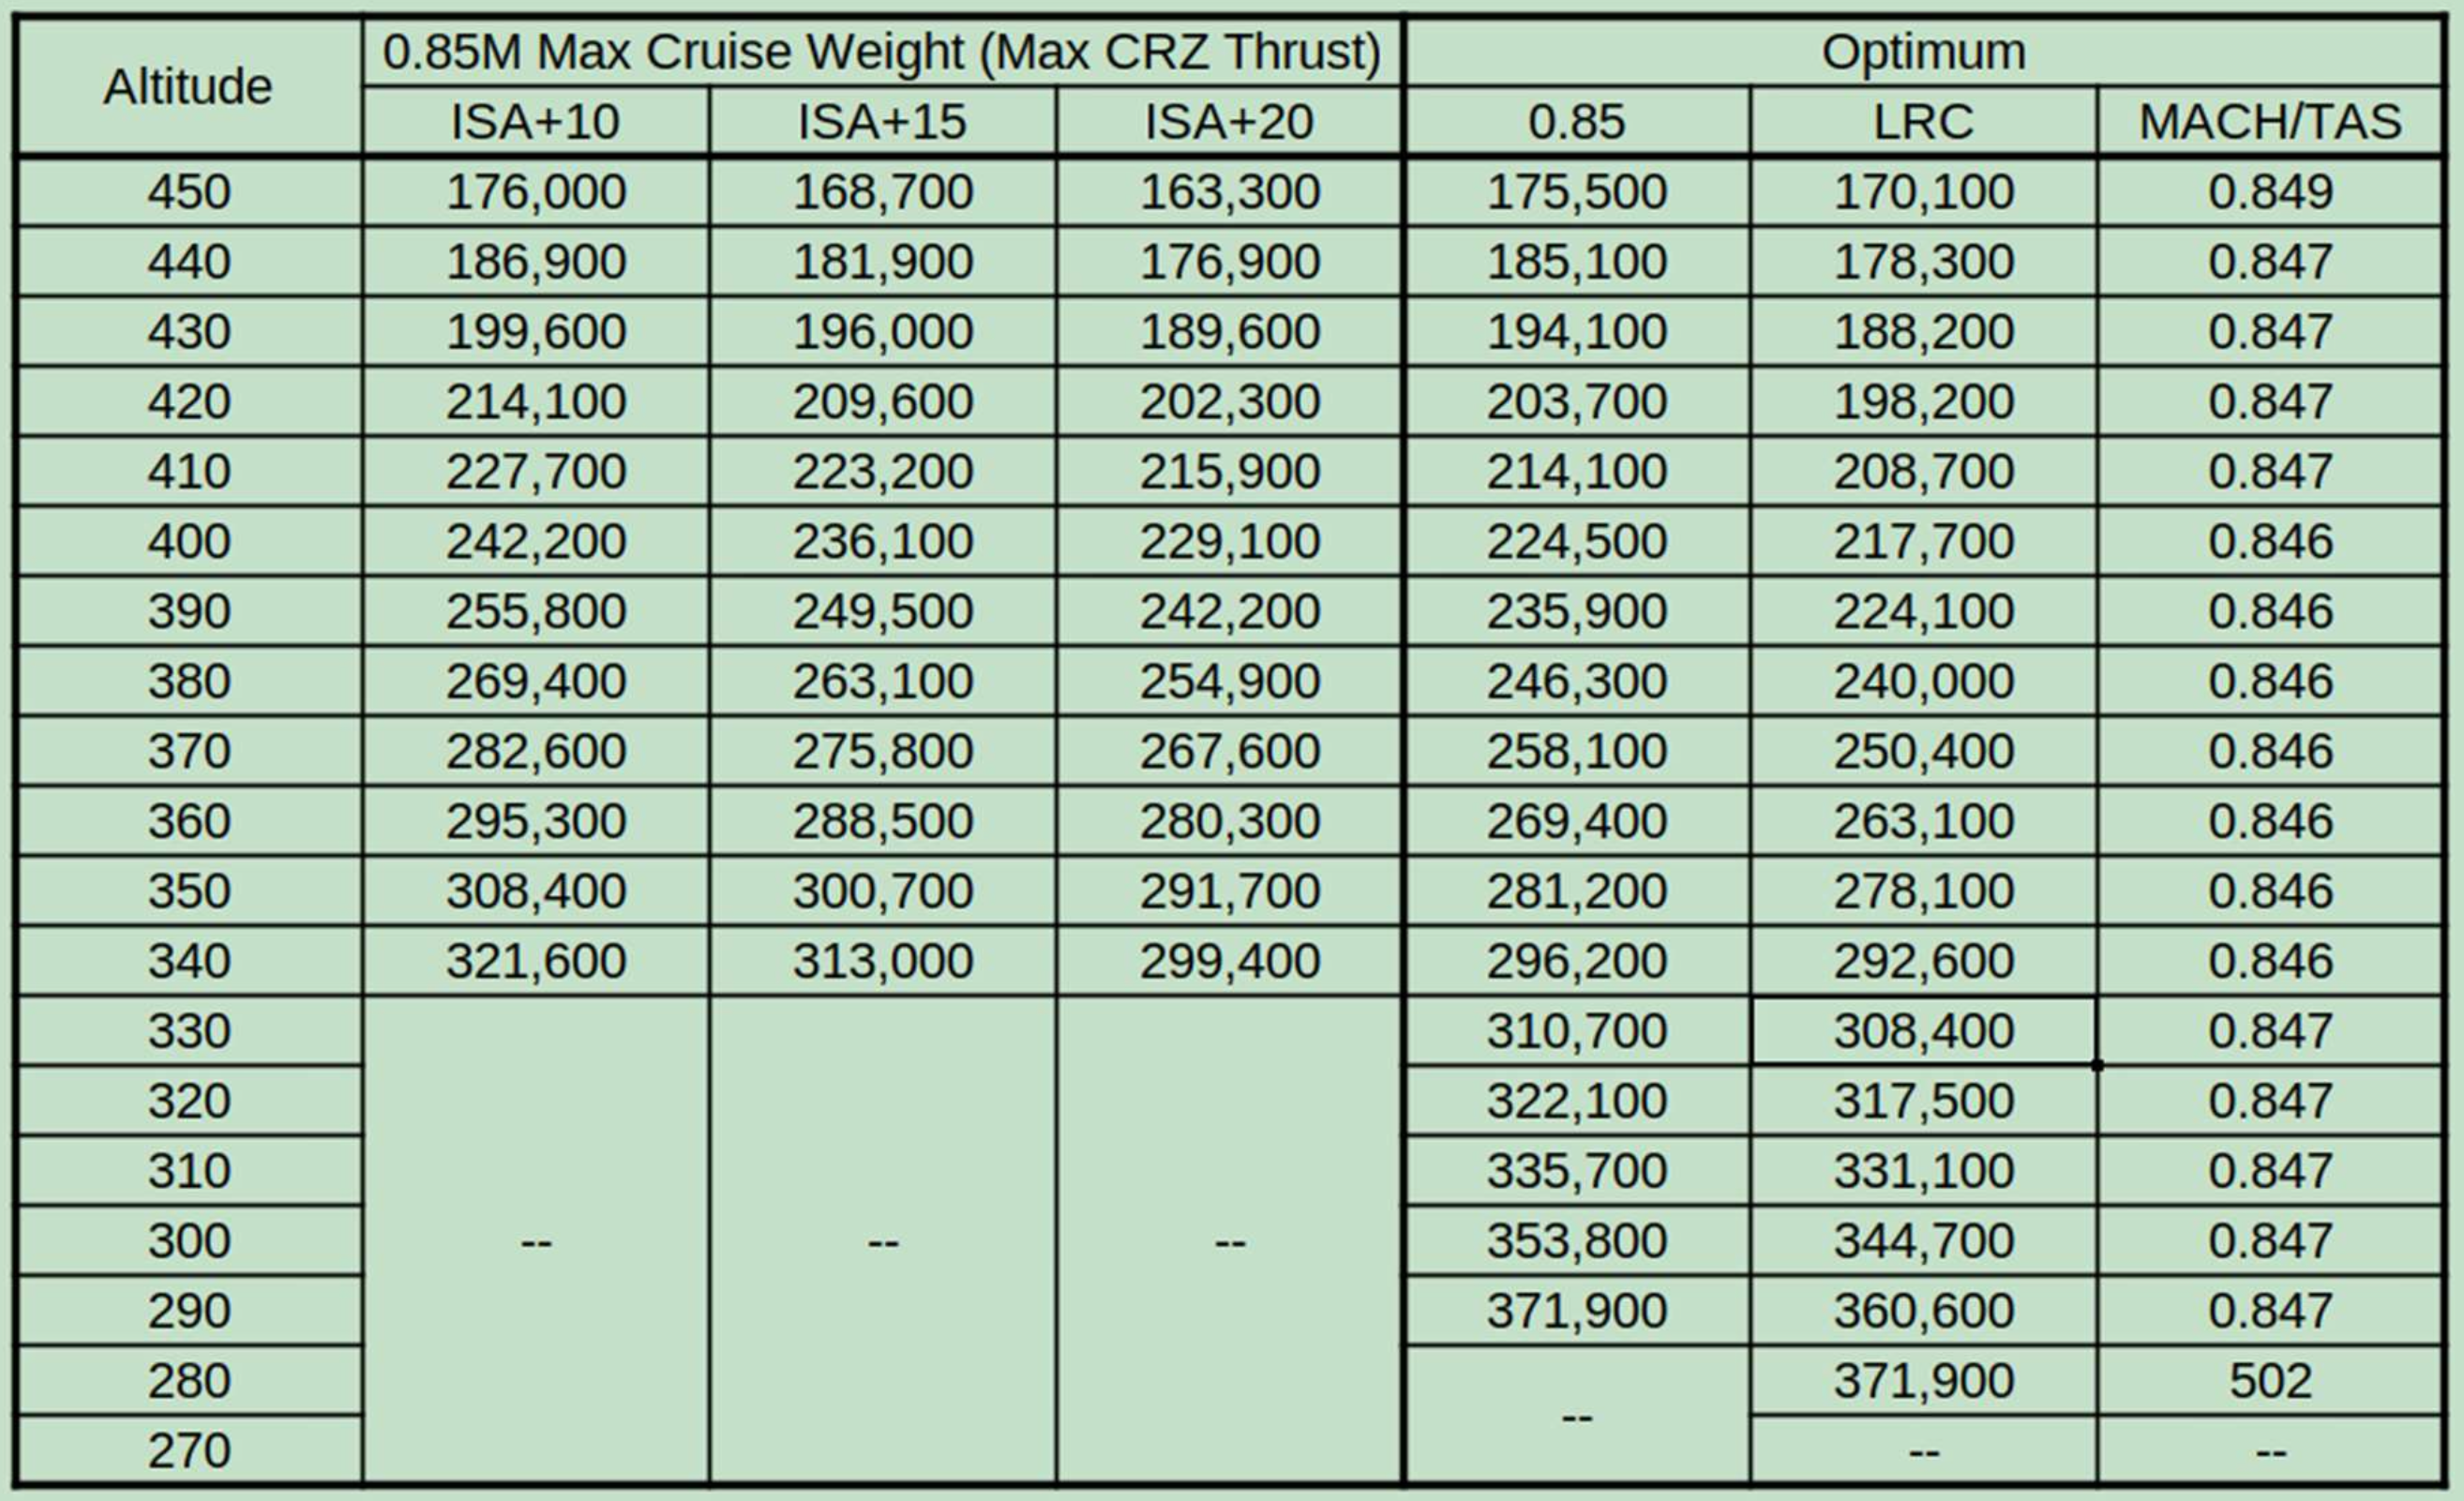
\includegraphics[width=\linewidth]{addenda/maxaltitude_kg_felis.png}
    \caption{Maximum \& Optimum Cruise Altitudes for Gross Weights in Kilogram}
\end{figure}

\begin{figure}[ht]
    \centering
	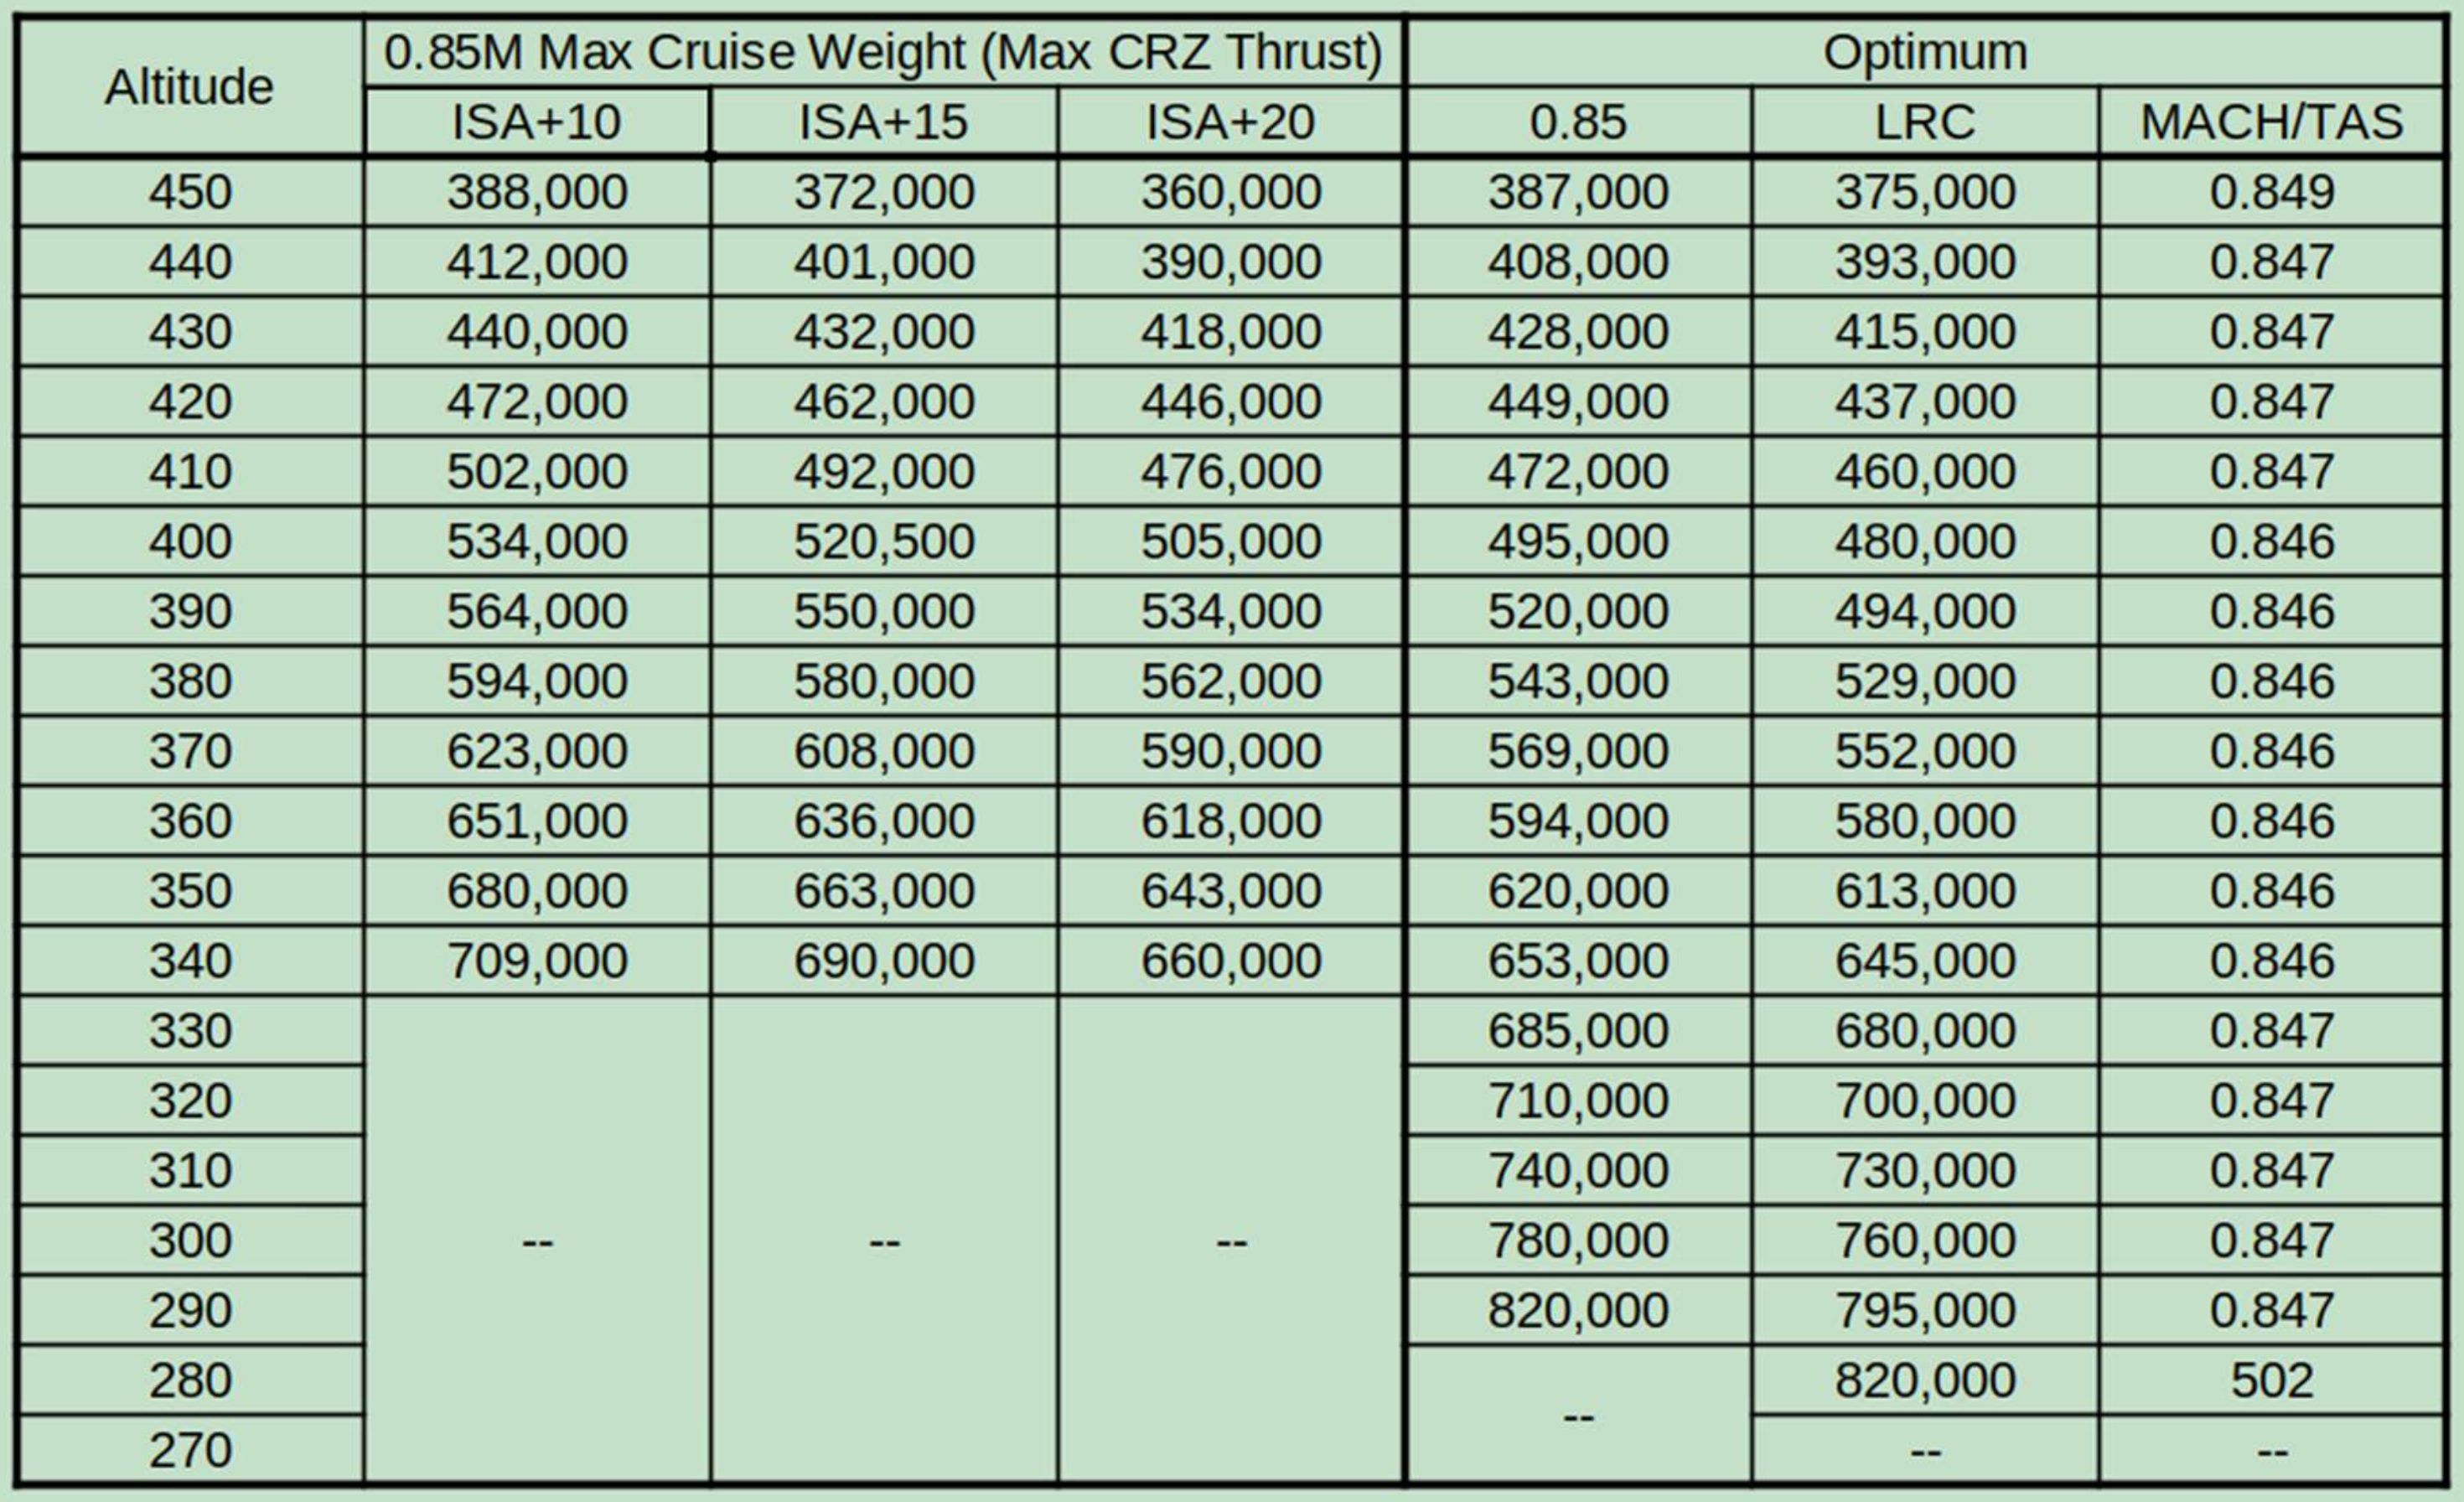
\includegraphics[width=\linewidth]{addenda/maxaltitude_lb_felis.png}
    \caption{Maximum \& Optimum Cruise Altitudes for Gross Weights in Pounds}
\end{figure}

\begin{figure}[ht]
    \centering
	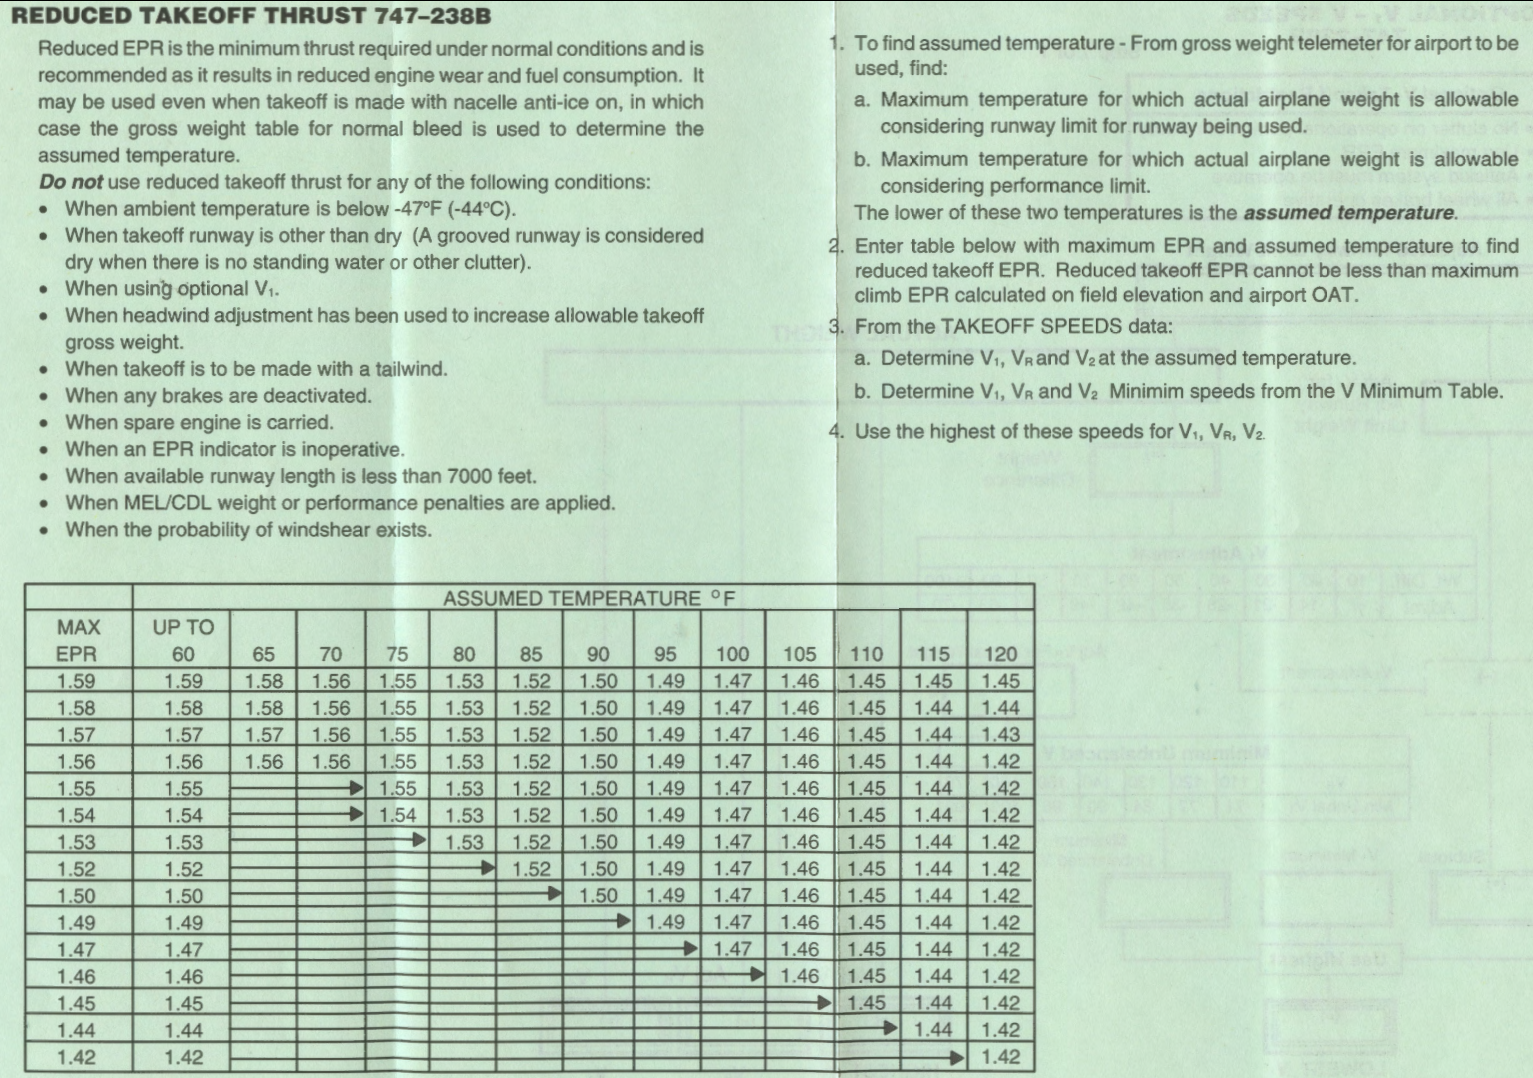
\includegraphics[width=\linewidth]{addenda/assumed_temp_742.png}
    \caption{EPR from Assumed Temperature, $^\circ F =\ ^\circ C \cdot 1.8 + 32$}
\end{figure}

\end{document}